Numerical solutions to problems in quantum physics are important, given the limited availability of exact solutions. Many such models and methods exist when dealing with many-body systems, and have been shown to provide good estimates of physical behaviour~\cite{BK:Krauth_2006}. Techniques such as Monte Carlo methods, exact diagonalisation, and DMRG are used to solve a wide variety of many-body problems, but often fail to capture the full system dynamics of such problems~\cite{NUM:Schollwock_rmp_2005}. For understanding the behaviour of systems such as Bose--Einstein condensates, the use of these methods is rather limited. For DMRG, the complexity of the problem grows quickly with increasing dimensionality and renders this technique unusable. Exact diagonalisation requires a linearised system to obtain realistic solutions, and also grows significantly in complexity with increased dimensionality. Monte Carlo methods generally do not allow for real-time dynamics, or reproducing the underlying wavefunction.

To obtain solutions to BEC problems we make use of a mean-field approach, outlined previously in Sec.~\ref{sub:gpederiv}. Using the GPE and performing a numerical integration allows for almost all examinable dynamics that are valid in the mean-field limit. It can be noted though that the computational cost increases significantly with increased dimensions, and is already non-trivial for two-dimensions. The following chapter will introduce the necessary requirements to numerically solve quantum problems using state-of-the-art computational methods.

We will begin with an introduction to the time evolution of a quantum state. We then discuss the use of the time evolution approach to find the ground state of a quantum system using imaginary time evolution. After this necessary mathematical introduction we will discuss the implementation of both real and imaginary time evolution using the Fourier split-operator (split-step) algorithm. We give error bounds for the algorithm, and discuss its use in the context of solving for Hamiltonian dynamics. Though the discussed algorithm is well suited to solving quantum dynamics, the computational cost can be quite high, especially for systems with large grid sizes.

We next discuss ways to overcome this through the use of high performance computing methods, and introduce the concept of graphical processing unit (GPU) computing. We present many of the necessary considerations for mapping a computational problem onto GPUs. Making use of GPUs to numerically solve the Schr\"odinger equation with the Fourier split-operator method, we present the problem of coherent atomic transport. We introduce the ``matter-wave spatial adiabatic passage'' technique, with the goal of coherently transporting an atom between trapping potentials with high fidelity. The design of the model system is presented, and the results are shown.

We finish the chapter by introducing the developed algorithms for condensate systems. Performance metrics and considerations are given in the context of solving the Gross--Pitaevskii equation in the presence of vortices.

\section{Time evolution}\label{sec:timeev}
Given a quantum state, to examine the dynamics requires an understanding of how it evolves in time. Assuming a quantum state at time $t_0$ to be defined as $|\Psi(t_0) \rangle$, and a state at time $t$ to be $|\Psi(t) \rangle$, the two states can be connected with a unitary evolution operator as
\begin{equation}
    |\Psi(t) \rangle = \mathscr{U}(t,t_0) | \Psi(t_0) \rangle,
\end{equation}
where we have assumed that $t > t_0$. One can write the wavefunction of a quantum system as the linear superposition of a set of basis states $|\Psi_m\rangle$ as
\begin{equation}\label{eqn:psicomplete}
    |\Psi \rangle = \displaystyle\sum\limits_{m} C_m |\Psi_m \rangle,
\end{equation}
with coefficients $C_m$. The unitary evolution operator can be written as
\begin{align}
   \mathscr{U}(t,t_0) &= \exp\left(-\frac{i\mathcal{H}(t - t_0)}{\hbar} \right) \\ &= \exp\left(\frac{-\text{i}\mathcal{H}\delta t}{\hbar}\right),
\end{align}
\iffalse
\begin{align}
   \mathscr{U}(t,t_0) &= \exp\left(-\frac{i}{\hbar}\displaystyle\int\limits_{t_0}^{t}\mathcal{H}\text{d}t\right),
\end{align}
\fi
where $\mathcal{H}$ is the Hamiltonian of the system, and $\delta t = t - t_0$. %For an incremental change $\delta t$ such that $t = t_0 +\delta t$ the above operator can be replaced by the form
%\begin{align}\label{eqn:timev_dt}
%   \mathscr{U}(t,t_0) &= \exp\left(\frac{-\text{i}\mathcal{H}\delta t}{\hbar}\right).
%\end{align}

The effect of $\mathscr{U}(t,t_0)$ on any arbitrary state can be examined by expanding it as
\begin{subequations}
    \begin{align}
        \mathscr{U}(t,t_0) &= 1 - \frac{\textrm{i}\mathcal{H}\delta t}{\hbar} + \mathcal{O}(\delta t^2) \\
        &= 1 - \frac{\textrm{i}\delta t}{\hbar}{\displaystyle\sum\limits_{n} E_n |\Psi_n\rangle \langle \Psi_n |} + \mathcal{O}(\delta t^2),
    \end{align}
\end{subequations}

where the Hamiltonian operator has been written as a complete set of energy eigenkets, $\mathcal{H}|\Psi_n\rangle = E_n|\Psi_n\rangle$. Applying this to \eqref{eqn:psicomplete} gives
\begin{subequations}
    \begin{align}
        |\Psi (t) \rangle &= \left( 1 - \frac{\textrm{i}\delta t}{\hbar}\displaystyle\sum\limits_{n}E_n|\Psi_n\rangle\langle \Psi_n |  \right)\displaystyle\sum\limits_{m} C_m |\Psi_m \rangle \\
            &= \displaystyle\sum\limits_{m} C_m |\Psi_m \rangle + \displaystyle\sum\limits_{n}\left( - \frac{\textrm{i}\delta t}{\hbar}E_n \right) C_n|\Psi_n\rangle,
    \end{align}
\end{subequations}
where terms of order $\mathcal{O}(\delta t^2)$ and higher have been temporarily left out for notational simplicity, but are still included in the analysis. Time evolving the state from $t_0$ to a final time $t$ by applying the evolution operator can then be written as
\begin{equation}
   \mathscr{U}(t,t_0)|\Psi(t_0) \rangle = \displaystyle\sum\limits_{n} C_n \exp\left(\frac{-\textrm{i}{E_n}\delta t}{\hbar}\right)|\Psi_n \rangle.
\end{equation}
It follows from here that each state oscillates at a different rate, proportional to its eigenenergy; higher energy states will oscillate faster than those of lower energy. For a given set of states the dynamics and evolution of the quantum system can be fully determined for all times using the above evolution operation.

As systems will prefer to reside in the lowest energy state where they are most stable, it is often required to determine the ground state solution of a particular Hamiltonian. A common method for this is by evolving the system in imaginary time. Taking the evolution operator, and applying a Wick rotation \cite{NUM:Bader_jcp_2013} rotates the time component through $\pi/2$ into the imaginary plane, as $t \rightarrow -it$. This new evolution operator applied to the wavefunction gives
\begin{equation}
       \mathscr{U^{'}}(t,t_0)|\Psi \rangle = \displaystyle\sum\limits_{n} C_n \exp\left(\frac{-{E_n}\delta t}{\hbar}\right)|\Psi_n \rangle.
\end{equation}
This process removes the complex term in the operator, which now takes the form of sums of exponentially decaying states. When applied to the wavefunction the higher energy terms will decay at a rate faster than lower energy components increasing $\delta t$. This process also causes a loss of probability density, and so the wavefunction must be renormalised after each application. Through repeated application of this operator, and a renormalisation afterwards, the simulated quantum system converges to the ground state solution. To begin, however, we must make an initial guess for the wavefunction, which has some finite overlap with the lowest lying state. It should be noted that this method is a mathematical trick used to obtain a simulated ground state, with a real-world system only tending to the ground state in the presence of some form of dissipation. As effective as this technique is, the convergence to the lowest lying energy state becomes less effective as the computation approaches the expected value \cite{Vtx:Danaila_pra_2005}, and if many eigenstates are lying close to each other. To ensure the system converges to a sufficient degree the resulting energy can be checked after each iteration, and the evolution stopped only when the energy change fluctuates about a stable value.

With the time evolution method introduced, we will next discuss implementing this method. Although many such algorithms exist to implement time evolution, one that is well suited for this task is the Fourier split-operator method. This method works equally for real, as well as imaginary, time evolution.

\section{Fourier split-operator method}\label{sec:fso}
The Gross--Pitaevskii equation is a second order nonlinear partial differential equation, and so very few exact solutions exist; the problem must often be tackled by a numerical approach. Though there are many ways to solve such a system numerically, with the Crank--Nicolson and Trotter--Suzuki algorithms being notable examples, the method we have chosen is the pseudospectral Fourier split-operator method, described below~\cite{Num:Bauke_cpc_2011}.

If we consider a unitary evolution operator of the form
\begin{equation}\label{eqn:1}
\Psi(\mathbf{x},t+\tau) = \exp\left( -\frac{\text{i}\hat{H}\tau}{\hbar}\right)\Psi(\mathbf{x},t),
\end{equation}
where $\hat{H}$ is the Hamiltonian, composed of momentum, potential, nonlinear interaction, and rotation terms defined in Eq. \eqref{eqn:gpe}, we can solve for the wavefunction, and its resulting dynamics over a specified timescale, assuming $\tau$ is a short time such that Eq.~\eqref{eqn:timev_dt} is valid. Care must be taken during the implementation of such integration methods, as the loss of precision due to floating-point rounding, as well as the propagation of errors cannot be neglected. If we take $\hat{H}$ in terms of its components as a combination of position and momentum space operators we obtain
\begin{equation}\label{eqn:2}
\hat{H} = \hat{H}_{\textbf{r}} + \hat{H}_{\textbf{k}} + \hat{H}_{\textbf{L}},
\end{equation}
where we first ignore the angular momentum operator, $\hat{H}_{\textbf{L}}$, and consider only the two other non-commuting parts, $\hat{H}_{\textbf{r}}$, containing the operators acting in position space, and $\hat{H}_{\textbf{k}}$, containing the operators acting in momentum space only. The Baker--Campbell--Hausdorf formula \cite{NUM:Weyrauch_cpc_2009} gives the relation for non-commuting operators as
\begin{equation}
    \exp\left( \tau(A+B) \right) = \exp\left(\tau A\right)\exp\left(\tau B\right)\exp\left(-\frac{\tau^2}{2}[A,B] + \cdots\right),
\end{equation}
with $\cdots$ representing higher order commutators. This is directly mappable to the above Hamiltonian for time evolution. Due to the non-commutativity of $\hat{H}_{\textbf{r}}$ and $\hat{H}_{\textbf{k}}$, the above expression cannot be evaluated exactly, and so it is common to Taylor expand and truncate it. The resulting error can be determined as
\begin{subequations}\label{eqn:error_calc}
\begin{align}
    \text{err} = \left\| \exp\left(-\frac{\textrm{i}\hat{H}_{\textbf{k}}\tau}{\hbar}\right)\exp\left(-\frac{\textrm{i}\hat{H}_{\textbf{r}}\tau}{\hbar}\right) - \exp\left(-\frac{\textrm{i}(\hat{H}_{\textbf{k}} + \hat{H}_{\textbf{r}})\tau}{\hbar}\right) \right\| \\
    = \left\|  \left(1 + \left(\frac{-\textrm{i}\hat{H}_{\textbf{k}}}{\hbar}\right)\tau + \left(\frac{-\textrm{i}\hat{H}_{\textbf{k}}}{\hbar}\right)^2\frac{\tau^2}{2}  \right)\left(1 + \left(\frac{-\textrm{i}\hat{H}_{\textbf{r}}}{\hbar}\right)\tau + \left(\frac{-\textrm{i}\hat{H}_{\textbf{r}}}{\hbar}\right)^2\frac{\tau^2}{2}  \right) \right. &- \nonumber \\ \left. \left(1 + \left(\frac{-\textrm{i}(\hat{H}_{\textbf{r}} + \hat{H}_{\textbf{r}})}{\hbar}\right)\tau + \left(\frac{-\textrm{i}(\hat{H}_{\textbf{r}} + \hat{H}_{\textbf{r}})}{\hbar}\right)^2\frac{\tau^2}{2}  \right)  + \mathcal{O}(\tau^3) \right\|,
\end{align}
\end{subequations}
which, upon simplification reduces to
\begin{equation}
\text{err} = \left\| \frac{\tau^2[{\hat{H}_{\textbf{r}}},{\hat{H}_{\textbf{k}}}]}{2\hbar^2} + \mathcal{O}(\tau^3)\right\| = \mathcal{O}(\tau^2).
\end{equation}

The error can be further reduced through the use of 2$^{\text{nd}}$ order Strang splitting~\cite{NUM:Gradinaru_SIAM_2007}, taking the error in the numerical integration scheme to $\mathcal{O}(\tau^3)$, with the resulting operator implementation given as

\begin{equation}\label{eqn:3}
\exp\left( -\frac{ \textrm{i}\left(\hat{H}_{\textbf{r}} + \hat{H}_{\textbf{k}}\right)\tau}{\hbar} \right) = \exp\left(- \frac{\textrm{i}\hat{H}_{\textbf{r}}\tau}{2\hbar} \right)\exp\left(-\frac{\textrm{i}\hat{H}_{\textbf{k}}\tau}{\hbar}\right)\exp\left( -\frac{\textrm{i}\hat{H}_{\textbf{r}}\tau}{2\hbar}\right) + \mathcal{O}\left(\tau^3\right).
\end{equation}
In the case of a nonlinear system, such as for solving the GPE, the above scheme attains a second-order error, resulting from the combination of the potential and nonlinear terms, with the respective mapping as \cite{BEC:Javanainen_jphysa_2006}
\begin{subequations}
    \begin{align}
\hat{H}_{\textbf{r}} &= V(\mathbf{r}) + g\vert\Psi(\mathbf{r},t)\vert^2, \\ \hat{H}_{\textbf{k}} &= \frac{-\hbar^2}{2m}\nabla^2.
    \end{align}
\end{subequations}
%\hat{H}_{\textbf{L}} = \Omega L,
Following Bauke \textit{et al}. \cite{Num:Bauke_cpc_2011}, we can numerically solve this differential equation as
\begin{equation}\label{eqn:baukeetal}
\Psi\left(\textbf{r},t+\tau\right) = \left[\hat{U}_{\mathbf{r}}\left(\frac{\tau}{2}\right) \mathscr{F}^{-1} \left[ \hat{U}_{\mathbf{k}}(\tau) \mathscr{F} \left[ \hat{U}_{\mathbf{r}}\left(\frac{\tau}{2}\right) \Psi\left(\mathbf{r},t\right) \right] \right] \right]  \\ + \mathcal{O}\left(\tau^2\right),
\end{equation}
where $\hat{U}_{\mathbf{r}}(\tau)=e^{-\textrm{i}\hat{H}_{\mathbf{r}}t/\hbar}$ is the time evolution operator in position space, $\hat{U}_{\mathbf{k}}(\tau)=e^{-i\hat{H}_{\mathbf{k}}t/\hbar}$ the time evolution operator in momentum space, and $\mathscr{F}$ and $\mathscr{F}^{-1}$ are the forward and inverse Fourier transform respectively. Taking the Fourier transform of the wavefunction allows the basis to be transformed between position and reciprocal space, wherein the time evolution operators are diagonal in each respective space. Figure~\ref{fig:num_splitop} outlines a schematic representation of the method during a single pass of the algorithm.

\begin{figure}
    \centering
    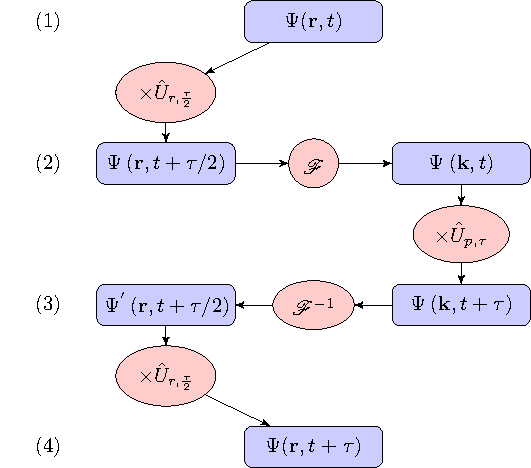
\includegraphics[]{./ch3_numerics/splitop}
    \caption{A single pass through the Fourier split-operator method.}
    \label{fig:num_splitop}
\end{figure}

The underlying theory of the Fourier split-operator method for the Gross--Pitaevskii equation is given by Javanainen \textit{et al}. \cite{BEC:Javanainen_jphysa_2006}, showing how the choice of nonlinearity and operator splitting affects the outcome of the method. By taking the initial step as evolution in momentum space, the choice of the most current wavefunction attains an error of third-order for the algorithm. However, this will require an additional two Fourier transform steps, and as such is rather costly in compute time for large systems. For an initial step in position space, the nonlinear term is best calculated using a linear combination of all available wavefunctions through the algorithm as $\Psi = c_0\Psi_0 + c_1\Psi_1 + c_2\Psi_2$, where the subscripts denote the wavefunction at each stage of the evolution in position space, as indicated in Fig.~\ref{fig:num_splitop}, and $c_{\textrm{x}}$ are linear coefficients for the states. This gives third order accuracy for the parameters $c_2=\pm 1, c_1=-c_0$. However, for simplicity and resource limitations we chose to work with the $\mathcal{O}\left(\tau^2\right)$ accurate scheme as depicted by Eq.~\eqref{eqn:baukeetal}, which was sufficient for the physics we aimed to describe.

An implementation of this method is a straight-forward process using MATLAB, and has been performed for the purpose of this study. However, due to the computational overhead required to time-evolve such a system, the procedure takes a long time to simulate at the required degree of accuracy for any dimension greater than one. Therefore, it is necessary to further develop the methods used, and to improve the implementation of this algorithm to leverage the recent advances in computational acceleration.

\subsection{Resolution considerations}
As the Fourier split-operator method requires special consideration of resolution in both position and momentum space, care must be taken while choosing numerical grids. The reciprocal relationship between position and momentum space is \begin{equation}
    k_{\text{max}} = \frac{2\pi}{\Delta x},
\end{equation}
which follows directly from the uncertainty relation; better resolution in one space leads naturally to worse in the other. To allow for a condensate to be simulated efficiently in both spaces, it must fit within the grid on which it is defined, and resolve to at least half the size of the smallest structure. It is easy to estimate a radius for the position space wavefunction, following the Thomas--Fermi approximation. It is also rather easy to know that for a non-rotating condensate the wavefunction should occupy the lowest lying mode ($\mathbf{k}=0$), and those close to it, assuming a harmonic trap. Rotating the condensate, however, has the effect of expanding the wavefunction in position space due to centrifugal forces. Additionally, the momentum space wavefunction also expands with increased angular momentum. With the addition of vortices to the system, there are now small scale structures to resolve. This leads to a system that is difficult to simulate; we have a simultaneously growing position space and momentum space wavefunction.

For a grid to effectively sample the wavefunction and capture all dynamics it will require a sampling rate of at least twice the smallest feature size following the Nyquist sampling theorem~\cite{BK:NumRecipes}. From this it is essential to have a large and finely sampled grid in order to resolve both position and momentum of the wavefunction, with all included features. For the simulations presented below a minimum grid size on the order of $2^8 = 256$ for low rotation rates, to $2^{11} = 2048$ at high rotation rates in 2D for both $X$ and $Y$ dimensions is necessary to correctly resolve the system dynamics in both position and momentum space with vortices present. One such way of ensuring accurate resolution of the system is to define a sufficient smallest length scale on one such grid (such as position). By ensuring the position grid remains defined with the same lowest increment, it is possible to increase resolution in the reciprocal space with a larger grid. As vortex core sizes are on the order of $\mu$m, the above parameters allow between sub-$\mu m$ ($2^{10}$ and above) to few $\mu m$ resolution. This also holds true for features in $\mathbf{k}$-space. Computationally, this can be costly, but quite effective when using compute accelerators (GPUs), which we will introduce next. %For the purpose of the work carried out herein, unless otherwise specified the simulations were resolved on a grid of $2^{10}\times 2^{10}$ elements, with spatial extent of the condensate $R\approx 700~\mu$m, and reciprocal space extent $K \approx 5\times10^{8}$ m$^{-1}$.
